\icode{E-MM-CA-L4-261014-001}
如图所示，一个质量为\(M\)，半径为\(R\)的光滑均质半球，静置于光滑水面上，在球顶有一个质量为\(m\)的质点，由静止开始沿球面下滑。试求：点离开球面以前的轨迹。

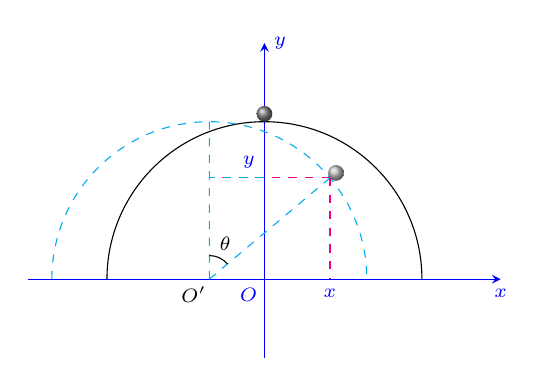
\begin{tikzpicture}[>=stealth,font=\scriptsize]
	\draw[->,blue] (-3,0)--(3,0)node[below]{\(x\)};
    \draw[->,blue] (0,-1)--(0,3)node[right]{\(y\)};
    \node at(-.2,-.2)[blue]{\(O\)};
	\draw (-2,0) arc(180:0:2);
	\shade[ball color=gray] (0,2.1) circle(.1);
	\begin{scope}[xshift=-.7cm]
	\draw[dashed,cyan] (-2,0) arc(180:0:2) (0,0)--(40:2) (0,0)--(0,2);
	\draw (0,.3) arc(90:40:.3);
	\draw[dashed,magenta] (40:2)--(0,{2*sin(40)}) (40:2)--({2*cos(40)},0)node[below,blue]{\(x\)};
	\node at(.7,{2*sin(40)+.2})[left,blue]{\(y\)};
	\shade[ball color=gray!50] (40:2.1) circle(.1);
	\node at(.2,.45) {\(\theta\)};
	\node at(-.2,-.2) {\(O^\prime\)};
	\end{scope}
	\draw[dashed,cyan] (0,{2*sin(40)})--(-.7,{2*sin(40)});
\end{tikzpicture}
\begin{answer}
   	\(\frac{x^2}{(\frac{MR}{M + m})^2} + \frac{y^2}{R^2} = 1\) 
\end{answer}